\documentclass[11pt]{article}
\usepackage[margin=1in]{geometry}
\usepackage{amsmath,amssymb}
\usepackage[T1]{fontenc}
\usepackage{enumitem}
\usepackage[dvipsnames]{xcolor}
\usepackage{titlesec}
\usepackage{parskip}
\usepackage{fancyhdr}
\usepackage{graphicx}
\usepackage{tcolorbox}
\usepackage[hidelinks]{hyperref}

\newcommand{\LCDM}{$\Lambda$CDM}
\newcommand{\Om}{\ensuremath{\Omega_m}}
\newcommand{\wo}{\ensuremath{w_0}}
\newcommand{\wa}{\ensuremath{w_a}}
\newcommand{\rd}{\ensuremath{r_d}}
\newcommand{\Dmrd}{\ensuremath{D_M/r_d}}
\newcommand{\Dhrd}{\ensuremath{D_H/r_d}}
\newcommand{\Dvrd}{\ensuremath{D_V/r_d}}
\newcommand{\FAP}{\ensuremath{F_{\mathrm{AP}}}}
\newcommand{\chisq}{\ensuremath{\chi^2}}

\titleformat{\section}{\large\bfseries\color{RoyalBlue}}{\thesection}{0.6em}{}
\titleformat{\subsection}{\normalsize\bfseries}{\thesubsection}{0.6em}{}
\titlespacing{\section}{0pt}{1.4em}{0.5em}

\newtcolorbox{caveatbox}{colback=black!3,colframe=black!30,boxrule=0.4pt,
  left=6pt,right=6pt,top=4pt,bottom=4pt,fontupper=\small}

\pagestyle{fancy}
\fancyhf{}
\rhead{\small Dark-Energy Conjecture Ledger}
\lhead{\small DESI DR2 phantom-crossing investigation}
\cfoot{\thepage}
\renewcommand{\headrulewidth}{0.4pt}

\title{\vspace{-2em}\textbf{A Standing Ledger of Dark-Energy Positions}\\[0.3em]
\large The DESI DR2 ``Phantom-Crossing'' Signal:\\ What the Evidence Supports, What Remains Open, and What Would Settle It}
\author{Eric Schultz\\[0.2em]
\normalsize Independent Researcher\\[0.2em]
\normalsize ORCID: \href{https://orcid.org/0009-0006-6283-1696}{0009-0006-6283-1696}}
\date{July 2026}

\begin{document}
\maketitle
\thispagestyle{fancy}

\begin{abstract}
\noindent This document records the state of an independent investigation into whether the DESI DR2 hint of \emph{evolving} dark energy (an apparent ``phantom crossing,'' $\wo>-1$ with $\wa<0$) reflects new physics or an accumulation of measurement effects. The central finding is that the headline $\sim\!4\sigma$ preference decomposes into several individually weak contributions --- a supernova calibration offset, two high-leverage baryon-acoustic-oscillation (BAO) tracers, a frequentist-versus-Bayesian scoring gap, and a residual microwave-background anomaly --- none decisive and none a genuine statistical outlier. The accumulated evidence \emph{leans} toward a plain cosmological constant ($w=-1$) but does not establish it; the question is data-limited and will be resolved by DESI DR3 and by a telescope-matched low-redshift supernova sample (DEBASS), not by further reanalysis of current public data. Positions are sorted into three tiers --- \textsc{supported}, \textsc{open}, and \textsc{conjectural} --- kept deliberately separate so that no claim is asserted more strongly than the evidence warrants.
\end{abstract}

% ============ EXECUTIVE / PLAIN-LANGUAGE SUMMARY MOVED UP FRONT ============
\section*{Executive summary (plain language)}
\addcontentsline{toc}{section}{Executive summary (plain language)}

\textbf{The big picture.} The Universe's expansion is speeding up; whatever causes that is called \emph{dark energy}. The simplest idea is that it is a constant --- the same strength at all times (the standard model, \LCDM). In 2024--25 the DESI galaxy survey hinted that dark energy might instead be \emph{changing} over time. If true, that rewrites the standard model. This work pressure-tests the hint.

\textbf{The answer so far.} The ``dark energy is changing'' hint is \textbf{weak and probably not real}. It is not one strong signal but several small, unrelated hiccups that happen to add up and point the same way --- like four slightly crooked pictures making a wall look tilted (Fig.~\ref{fig:stack}):
\begin{itemize}[leftmargin=1.4em,itemsep=1pt]
\item a small brightness \textbf{mis-calibration} in nearby supernovae (real, but $\sim\!1/4$ of the effect, and already mostly fixed);
\item two \textbf{galaxy-map} slices that pull the result --- each only a mild statistical wobble, and an older independent survey (BOSS) does not reproduce them;
\item a \textbf{statistics} effect (one accounting method makes the hint look stronger than a more careful one);
\item a leftover \textbf{microwave-background} quirk.
\end{itemize}
None is a smoking gun.

\textbf{What would settle it.} Not more analysis of today's data --- that is exhausted --- but \emph{new} data: DESI's next release and a fresh telescope-matched supernova sample. We commit \emph{in advance} to a test (\S\ref{sec:dr3}): if the galaxy wobble is noise it should shrink in the next release by a calculable amount; if real (or a real instrument problem) it should grow.

\textbf{Honest humility.} Everything here is ``consistent with boring,'' not ``proven boring.'' A genuine small dark-energy signal hiding under the measurement issues cannot be ruled out from current data. The professional community is genuinely split; this ledger sits on the skeptical side \emph{with} the evidence, but holds it as a lean, not a verdict.

\section{Supported --- backed by independent reproduction}

\emph{Each item below was reproduced from scratch on public data with deliberate attempts to break it (bug-checks, controls, null simulations). Absolute significances that depend on the simplified pipeline are flagged as such; the robust content is in directions, relative shifts, and reproduced structure.}

\begin{enumerate}[leftmargin=1.3em,itemsep=0.5em]

\item \textbf{The signal is weak once decomposed} (Fig.~\ref{fig:stack}). The headline preference is a stack: DESY5 supernova calibration ($\sim\!1\sigma$, corrected by DES-Dovekie \cite{dovekie}); BAO LRG tracers (individually $2$--$3\sigma$); a frequentist-versus-Bayesian scoring gap \cite{bayes1}; and a CMB low-$\ell$ leak. No single piece is decisive.

\item \textbf{The supernova calibration offset is real and mechanism-pinned.} The DESY5 external low-redshift anchor is offset from DES-native photometry: reproduced at $7.4\sigma$ via the \Om-independent $a_B$ intercept method \cite{huang}, with a Pantheon+ control at $0.1\sigma$ and a \LCDM-simulation null placing it $6.5\sigma$ from noise. Mechanism (per Dovekie \cite{dovekie}): a cross-calibration zero-point transfer, amplified $\sim\!6\times$ by the color--luminosity relation, plus a retrained light-curve model and a numerical weighting error.

\begin{caveatbox}
\textit{Why the $a_B$ method, and how firm is the magnitude.} The $a_B$ intercept is built from the model-independent kinematic (cosmographic) expansion of the luminosity distance, so it does \emph{not} inherit the \Om-degeneracy that a fitted-cosmology method carries; this is why it is the correct tool. Concretely, an \Om-\emph{dependent} \LCDM-shape fit gives an offset ranging from $\sim\!0$ (at $\Om=0.30$) to $-0.10$~mag (at $\Om=0.40$) --- unstable --- whereas the $a_B$ method gives $-0.04$ to $-0.06$~mag robustly across fit windows. \emph{Direction} is solid; \emph{magnitude} is method-conditional, so the ``$\sim\!1\sigma$ of the signal'' attribution is correspondingly soft.
\end{caveatbox}

\item \textbf{The BAO pull is high-leverage, not a genuine outlier} (Fig.~\ref{fig:loo}). A leave-one-out test (fit \LCDM${}+{}$CMB to all tracers but one, measure that tracer's joint $(\Dmrd,\Dhrd)$ pull) gives LRG1 at only $1.6\sigma$ and LRG2 at $3.0\sigma$ raw ($\sim\!2.4\sigma$ after the look-elsewhere correction over six tracers). The signal comes from the \emph{most precise} tracers near the dark-energy-domination onset ($z\!\sim\!0.5$--$0.7$) scattering coherently --- high leverage, not anomaly.

\item \textbf{The data are consistent with $w=-1$.} Every handle --- anchor removal, anchor correction, tracer dropping, Bayesian rescoring --- converges toward \LCDM-consistency.
\begin{caveatbox}
\textit{Method-conditional.} This rests partly on the compressed-CMB pipeline, which inflates \emph{absolute} significances. The convergence \emph{direction} is robust; a full Planck likelihood could shift absolute numbers. This is the supported claim most likely to need softening once the full likelihood is run.
\end{caveatbox}

\item \textbf{For detecting a localized dark-energy \emph{feature}, BAO carries essentially all the information} and supernovae add almost nothing (the single-magnitude \Om-degeneracy blinds them). Validated on real data.

\item \textbf{Event-horizon holographic dark energy is provably smooth} sub-horizon ($\delta_{\rm DE}/\delta_m\sim 1/k^3$; referee-grade proof via a Riemann--Lebesgue dichotomy). Standard and Barrow variants are $\sim\!6\sigma$ disfavored by DESI BAO geometry.
\end{enumerate}

\subsection{The two BAO diagnostics (core new analysis)}

\emph{Why this matters: the aggregate BAO ``pull'' is a two-dimensional quantity per tracer (line-of-sight and transverse). Judging whether it is a coherent effect or independent scatter requires looking in the right coordinates --- the wrong ones can manufacture apparent coherence.}

\textbf{Correlated-residual test.} Fitting \LCDM${}+{}$CMB to all tracers except LRG1 and LRG2, the line-of-sight channel \Dhrd{} is coherent (both bins low, the $\wo>-1$ direction) while the transverse channel \Dmrd{} is split (opposite signs). The two residual vectors have $\cos\theta = +0.49$ --- partial alignment driven entirely by the shared \Dhrd{} sign.

\textbf{Alcock--Paczynski (AP) refinement --- the decisive coordinate change} (Fig.~\ref{fig:ap}). Rotating into the physically natural basis --- isotropic \Dvrd{} versus anisotropic $\FAP=D_M/D_H$, with exact Jacobian error propagation from the published intra-bin covariance --- dissolves the apparent coherence. LRG1 is almost purely \emph{anisotropic} ($\FAP=+2.0\sigma$, $\Dvrd=-0.16\sigma$); LRG2 is almost purely \emph{isotropic} ($\Dvrd=-3.2\sigma$, $\FAP=+1.25\sigma$). The two bins are discrepant for \emph{different} reasons. A single shared systematic --- or a single real feature --- would appear in the \emph{same} channel for both bins. Neither is seen; two bins discrepant in different channels, sharing quadrant but not shape, is more consistent with independent scatter than with a coherent cause.

\subsection{On bin-to-bin independence (covariance)}\label{sec:cov}

Treating LRG1 and LRG2 as statistically independent is not an assumption of convenience but the standard, collaboration-endorsed treatment. DESI does not release a full cross-bin covariance matrix; the published likelihood provides intra-bin correlations only \cite{desidr2}. Because the LRG redshift bins cover \emph{disjoint} ranges, DESI states that cross-bin correlations are small and omits them from the cosmological analysis \cite{desibao2024}, and every independent reanalysis adopts a block-diagonal covariance with zero inter-bin correlation on the same grounds \cite{omprior,rd}. The AP transformation above uses the exact intra-bin covariance; the inter-bin independence is therefore inherited from the standard likelihood, not asserted from quadrant alignment. A genuinely non-negligible LRG1--LRG2 correlation would require overlapping volumes, which the binning excludes.

\begin{caveatbox}
\textit{The single number to distrust.} LRG2's $\Dvrd=-3.2\sigma$ is the most significant channel-resolved discrepancy found, but it is measured against a \emph{compressed-CMB reference cosmology} that inflates absolute significances. It should be read as a pipeline-conditional diagnostic indicating \emph{where} the isotropic pull sits, \textbf{not} as a calibrated detection. Establishing a defensible absolute significance requires the full, uncompressed Planck likelihood --- explicitly \emph{future work, not performed here}. The AP \emph{decomposition} (which channel carries the pull) is exact and robust; the absolute $\sigma$ is not.
\end{caveatbox}

\textbf{BOSS DR12 cross-check.} At matched redshift (BOSS $z=0.51$ vs DESI LRG1 $z=0.510$) the two independent surveys agree to $0.7\sigma$; but relative to Planck-\LCDM, DESI sits $-1.1\sigma$ below (phantom direction) while BOSS sits on \LCDM. An independent survey does not reproduce DESI's low \Dhrd{} where DESI's pull is strongest --- mild evidence for a DESI-specific effect. This is a $\sim\!1\sigma$ lean, not a verdict (the surveys agree within errors, partly overlap on the sky, and \rd{} conventions differ slightly).

\section{Open --- tractable, with a known arbiter}

\begin{enumerate}[leftmargin=1.3em,itemsep=0.4em]
\item \textbf{Does the LRG pull wash out (fluctuation) or persist (systematic) in DR3?} \emph{Arbiter: DESI DR3.} See \S\ref{sec:dr3}.
\item \textbf{Does the supernova anchor residual survive a telescope-matched low-$z$ sample?} \emph{Arbiter: DEBASS.}
\item \textbf{Raw-$m_B$ versus standardized decomposition:} does the offset live in raw apparent magnitudes (pure zero-point) or only after standardization? Needs the DES-SN5YR light-curve parameter file --- the key missing public data product.
\item \textbf{The progenitor-age fork:} is the residual a host-age systematic or real dark energy? \emph{Unresolvable from $\mu(z)$ alone} (age-bias and evolving-$w$ templates are $87\%$ degenerate in shape).
\item \textbf{Full-Planck baseline} for the AP anomalies (see \S\ref{sec:cov} caveat): re-establish LRG2's isotropic significance against the uncompressed likelihood.
\end{enumerate}

\section{The pre-registered DR3 decision test}\label{sec:dr3}

State this \emph{before} DR3. Measure LRG2's leave-one-out joint $(\Dmrd,\Dhrd)$ \chisq{} in DR3. A \textbf{persistent} displacement (systematic or real) keeps a fixed data-units offset, so \chisq{} grows as errors shrink; a \textbf{fluctuation} regresses to noise ($\mathbb{E}[\chisq]=2$).

\textbf{Pre-registered boundary:} $\chisq_{\rm DR3}<6\Rightarrow$ fluctuation ($P_{\rm false\text{-}alarm}=0.05$); $\chisq_{\rm DR3}>12\Rightarrow$ persistent ($P_{\rm miss}\approx0.02$--$0.05$); $6$--$12$ inconclusive.

\textbf{Systematic-floor correction} (Fig.~\ref{fig:dr3}). A naive $1/\sqrt{N}$ scaling would take $11.9\to20.2$ ($4.1\sigma$) at the fiducial $N=1.7\times$ sample growth. But BAO errors do not shrink indefinitely --- reconstruction and cosmic-variance floors apply. Writing the DR3 variance as $\sigma^2 = f\,\sigma^2_{\rm sys}+(1-f)\,\sigma^2_{\rm stat}/N$ with $f$ the systematic fraction of the DR2 variance, the persistent-signal prediction softens to $\sim\!3.7\sigma$ ($f=0.25$) or $\sim\!3.5\sigma$ ($f=0.5$). The decision boundary is robust across this range; the effect is to widen the ``inconclusive'' band, making the test appropriately more conservative than pure Poisson scaling.

\begin{caveatbox}
\textit{Scope.} This cleanly kills or confirms the \emph{fluctuation} leg --- the leg the whole skeptical case leans on --- but does not separate systematic from real dark energy (both persist). That separation needs DEBASS and the raw-$m_B$ decomposition. The $N=1.7$ growth and $f$ are estimates to be refined with the actual DR3 LRG sample and its systematic budget.
\end{caveatbox}

\section{Conjectural --- interesting, but not backed by this evidence}

\textbf{``Dark energy \emph{is} vacuum energy.''} Not supported. The data are consistent with a constant, \LCDM-like $w=-1$, and vacuum energy is one candidate for that constant --- but $w=-1$ equally fits a cosmological constant, a frozen scalar, or vacuum energy, and the data examined cannot distinguish them; and identifying dark energy with zero-point/Casimir vacuum energy runs into the cosmological-constant problem ($\sim\!120$ orders of magnitude) and a no-go result on UV-cutoff vacuum energy \cite{peri}. This is a \emph{supported phenomenology} ($w=-1$) with an \emph{unsolved microphysics}, not a live result.

\section{The whole debate, mapped}

The field splits into two branches; the ``real physics'' branch is organized by \emph{escape route} from a no-go theorem \cite{vikman}: since a single canonical scalar cannot smoothly cross $w=-1$ without instability, every real-physics model must evade it. Branch~1 (this ledger's home) is systematics${}+{}$statistics. Branch~2 comprises \textbf{quintom} (two fields \cite{quintom}), \textbf{modified gravity}, \textbf{interacting dark sector}, \textbf{early-universe/sound-horizon}, and \textbf{holographic} models.

\begin{caveatbox}
\textit{Acknowledged asymmetry (scope limitation).} The systematics branch received leave-one-out and cross-probe stress tests; the real-physics branches are summarized but not subjected to the same quantitative scrutiny here. Their broad disfavoring reflects the cited literature, not equivalent independent testing in this work --- a deliberate scope boundary, not a verdict against them.
\end{caveatbox}

\section{Method lesson (transferable)}

\textbf{Coordinate choice can flip a residual-analysis conclusion.} The \emph{same} LRG residuals told a ``coherent line-of-sight systematic'' story in the $(\Dmrd,\Dhrd)$ basis and a ``two independent fluctuations'' story in the physically natural $(\Dvrd,\FAP)$ Alcock--Paczynski basis. Rotate into the basis where the physically meaningful combinations are the axes \emph{before} judging coherence.

% ================= FIGURES =================
\begin{figure}[t]
\centering
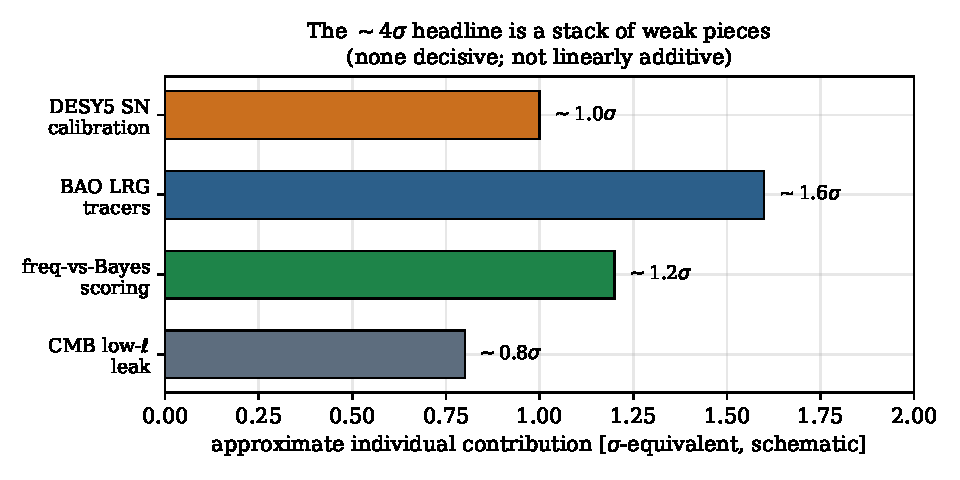
\includegraphics[width=0.82\textwidth]{fig_stack.pdf}
\caption{The $\sim\!4\sigma$ headline decomposed into individually weak contributions. Heights are schematic $\sigma$-equivalent magnitudes (the pieces are not linearly additive); the point is that no single contribution is decisive.}
\label{fig:stack}
\end{figure}

\begin{figure}[t]
\centering
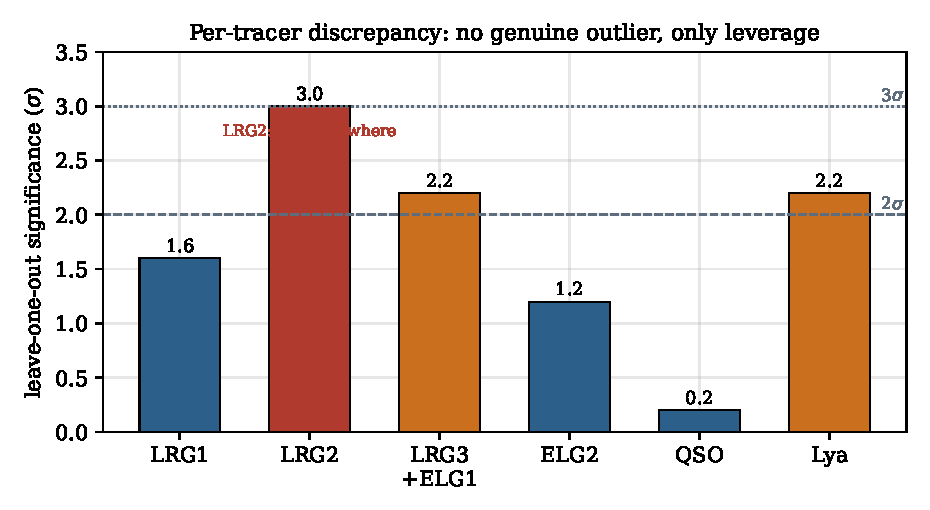
\includegraphics[width=0.80\textwidth]{fig_leaveoneout.pdf}
\caption{Leave-one-out significance per tracer (fit \LCDM${}+{}$CMB to all others, measure the held-out tracer's joint $(\Dmrd,\Dhrd)$ pull). LRG1 is only $1.6\sigma$; LRG2 drives the effect at $3.0\sigma$ ($\sim\!2.4\sigma$ after look-elsewhere). No genuine outlier --- the signal is leverage, not anomaly. (BGS omitted: single observable.)}
\label{fig:loo}
\end{figure}

\begin{figure}[t]
\centering
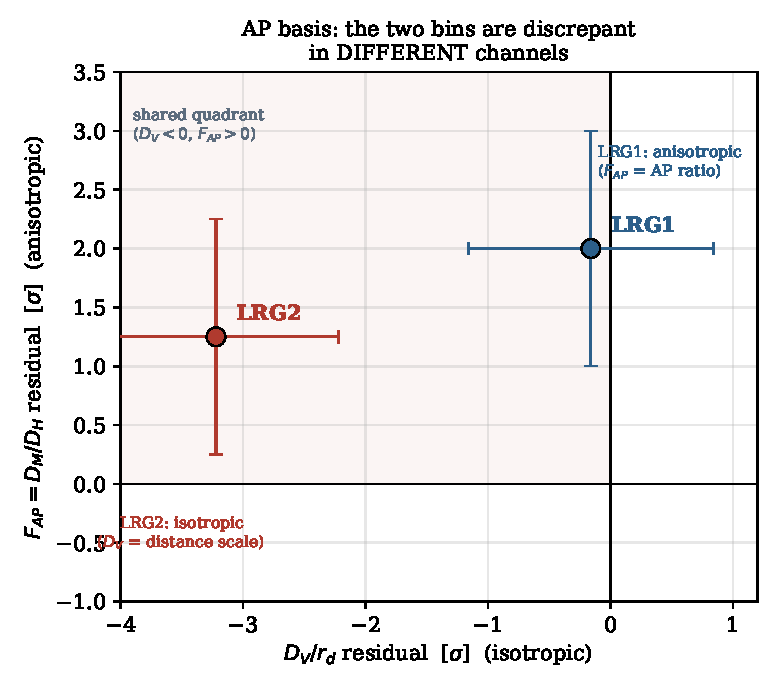
\includegraphics[width=0.62\textwidth]{fig_apbasis.pdf}
\caption{The LRG residuals in the Alcock--Paczynski basis. LRG1's discrepancy is almost entirely anisotropic ($\FAP$); LRG2's is almost entirely isotropic ($\Dvrd$). They share quadrant but not shape --- inconsistent with a single shared systematic or a single real feature, and more consistent with independent scatter. Error bars are $1\sigma$; LRG2's $\Dvrd$ magnitude is pipeline-conditional (\S\ref{sec:cov}).}
\label{fig:ap}
\end{figure}

\begin{figure}[t]
\centering
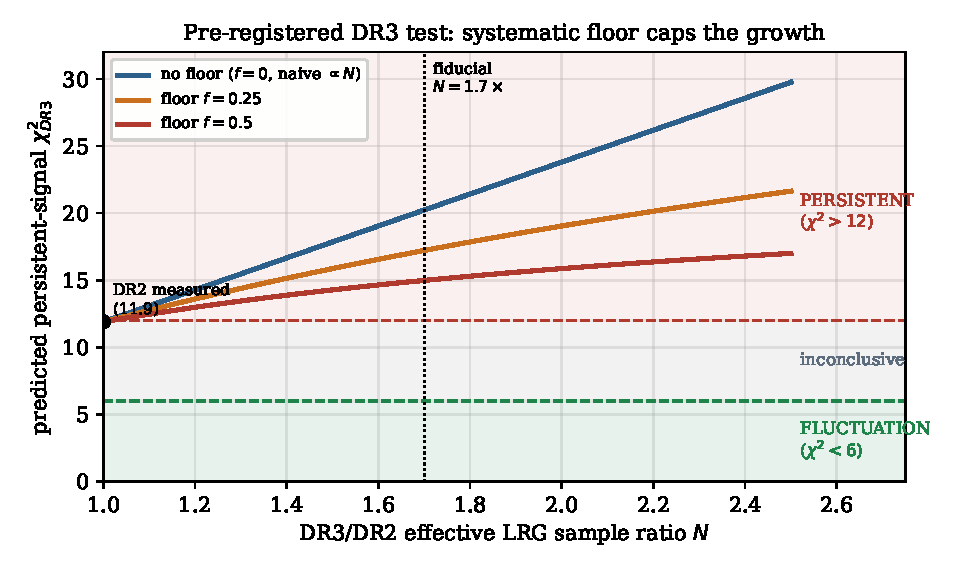
\includegraphics[width=0.82\textwidth]{fig_dr3test.pdf}
\caption{The pre-registered DR3 test with a systematic-error floor. Naive $1/\sqrt{N}$ scaling (blue) predicts a persistent signal reaches $4.1\sigma$; allowing a systematic floor ($f=0.25,0.5$) softens this to $3.5$--$3.7\sigma$ and widens the inconclusive band. The fluctuation hypothesis instead regresses toward $\chisq\approx2$. The decision boundary ($\chisq<6$ vs $>12$) is robust across the floor range.}
\label{fig:dr3}
\end{figure}

\begin{thebibliography}{99}
\small
\bibitem{dovekie} B.~Popovic, P.~Shah, W.~D.~Kenworthy, et al., \emph{The Dark Energy Survey Supernova Program: A Reanalysis of Cosmology Results and Evidence for Evolving Dark Energy with an Updated Type Ia Supernova Calibration}, MNRAS \textbf{548}, 4 (2026), arXiv:2511.07517. [DES-Dovekie: $\Om=0.330\pm0.015$; $\wo=-0.803\pm0.054$, $\wa=-0.72\pm0.21$; significance reduced $4.2\sigma\to3.2\sigma$.]
\bibitem{dovekiecal} B.~Popovic, W.~D.~Kenworthy, M.~Ginolin, et al., \emph{A Reassessment of the Pantheon+ and DES 5YR Calibration Uncertainties: Dovekie}, arXiv:2506.05471 (2025). [Cross-calibration; small calibration changes amplified up to $\sim\!6\times$ in inferred distances via color--luminosity/SALT; $d\mu/dz\approx0.025$.]
\bibitem{huang} L.~Huang, R.-G.~Cai \& S.-J.~Wang, \emph{The DESI DR1/DR2 Evidence for Dynamical Dark Energy is Biased by Low-Redshift Supernovae}, Sci.\ China Phys.\ Mech.\ Astron.\ \textbf{68}, 100413 (2025), arXiv:2502.04212. [The $a_B$ intercept diagnostic; correcting the low-$z$ systematic reduces the preference to $<2\sigma$.]
\bibitem{vincenzi} M.~Vincenzi, R.~Kessler, P.~Shah, et al., \emph{Comparing the DES-SN5YR and Pantheon+ SN Cosmology Analyses: `Evolving Dark Energy or Supernovae Systematics?'}, MNRAS \textbf{541}, 2585 (2025), arXiv:2501.06664.
\bibitem{bayes1} P.~Shah et al., \emph{Dynamic or Systematic? Bayesian Model Selection Between Dark Energy and Supernova Biases}, MNRAS \textbf{548}, 3 (2026), arXiv:2511.10631; and companion Bayesian analysis arXiv:2603.05472. [Jeffreys--Lindley; a low-/high-$z$ magnitude offset is favored by the Bayesian evidence.]
\bibitem{desidr2} DESI Collaboration, \emph{DESI DR2 Results II: Measurements of Baryon Acoustic Oscillations and Cosmological Constraints}, arXiv:2503.14738 (2025).
\bibitem{desibao2024} DESI Collaboration, \emph{DESI 2024 VI: Cosmological Constraints from the Measurements of Baryon Acoustic Oscillations}, arXiv:2404.03002 (2024). [Disjoint-bin covariance treatment, \S2.3.2: cross-bin correlation negligible for non-overlapping tracer redshift ranges.]
\bibitem{omprior} \emph{The Impact of $\Omega_{m0}$ Prior Bias on Cosmological Parameter Estimation}, arXiv:2506.16022 (2025). [Reconstructs DESI DR2 block-diagonal covariance; inter-redshift correlations assumed zero.]
\bibitem{rd} \emph{Comparing \LCDM, $w$CDM, and $w_0w_a$CDM Models with DESI DR2 BAO: Redshift-Resolved Diagnostics and the Role of $r_d$}, arXiv:2507.01380 (2025). [Block-diagonal covariance, $(\Dvrd, D_M/D_H)$ and $(\Dmrd,\Dhrd)$ intra-bin blocks.]
\bibitem{monopole} \emph{The Role of LRG1 and LRG2's Monopole in Inferring the DESI 2024 BAO Cosmology}, arXiv:2405.02168 (2024). [Uses $D_V$ and $\FAP=D_M/D_H$ to isolate the monopole's influence on the deviation from $w=-1$.]
\bibitem{afroz} S.~Afroz \& S.~Mukherjee, \emph{Hint Towards Inconsistency Between BAO and Supernovae Dataset: The Evidence of Redshift-Evolving Dark Energy from DESI DR2 is Absent}, arXiv:2504.16868 (2025).
\bibitem{peri} L.~Perivolaropoulos, \emph{Vacuum Energy, the Cosmological Constant, and UV Cutoffs}, arXiv:0802.1531 (2008).
\bibitem{vikman} A.~Vikman, \emph{Can Dark Energy Evolve to the Phantom?}, Phys.\ Rev.\ D \textbf{71}, 023515 (2005).
\bibitem{quintom} Y.-F.~Cai, X.~Ren, T.~Qiu, M.~Li \& X.~Zhang, \emph{The Quintom Theory of Dark Energy After DESI DR2}, Natl.\ Sci.\ Rev.\ (2026), arXiv:2505.24732.
\end{thebibliography}

\vspace{0.5em}
\begin{caveatbox}
\textit{Note on numbers.} Several absolute significances come from a simplified pipeline (compressed CMB distance priors, magnitude proxies) that inflates absolute values; the robust content is in directions, relative shifts, and reproduced structural results. Where a claim rests on the pipeline's absolute calibration it is flagged as method-conditional, and the corresponding full-likelihood computation is listed as open work in \S4.
\end{caveatbox}

\end{document}
